\documentclass[red]{beamer}

\mode<presentation>{
\usetheme{Boadilla}
\usecolortheme{default}
}
\usepackage{CJK}
\usepackage{graphicx}
\usepackage{amsmath, amsopn}
\usepackage[english]{babel}
\usepackage[latin1]{inputenc}
\usepackage{url}
\usepackage{color}
\usepackage{times}
\usepackage{xcolor}
\usepackage{listings}
\lstset{
language=bash,
keywordstyle=\color{blue!70}\bfseries,
basicstyle=\ttfamily,
commentstyle=\ttfamily,
showspaces=false,
showstringspace=false,
showtabs=false,
frame=shadowbox,
rulesepcolor=\color{red!20!green!20!blue!20},
breaklines=true}
\title[BI028]{BI028: Linux and Shell Programming}
\author[Maoying]{Maoying,Wu\\
{\scriptsize ricket.woo@gmail.com}}
\institute[CBB] % (optional, but mostly needed)
{
  \inst{}
  Dept. of Bioinformatics \& Biostatistics\\
  Shanghai Jiao Tong University
}
\date{Spring, 2016}

\AtBeginSubsection[]
{
  \begin{frame}<beamer>{Next we will talk about ...}
    \tableofcontents[currentsection,currentsubsection]
  \end{frame}
}

\begin{document}
\begin{CJK*}{GBK}{kai}
\frame{\titlepage}

\section[Outline]{Course Outline}
\begin{frame}
\frametitle{Course Overview}
\begin{itemize}
	\item \textbf{Course Description}: Linux command line, system administration and 
		bash/python programming
	\item \textbf{Prerequisite}: None
    \item \textbf{Textbook}: None
    \item \textbf{Grading}: Grades will be determined roughly by
    \begin{itemize}
        \item 5 Quizzes: 20\% total
        \item Take-home Practical Final: 30\%
        \item Assignments: 20\%
        \item Projects: 25\%
    \end{itemize}
    \item \textbf{Exams}: There will be 5 quizzes, 1 bring-home practical final.
        All exams will be open-book, and cover materials from lectures, discussions, 
		labs and extracurricular readings.

    \item \textbf{Webpage}: \url{http://cbb.sjtu.edu.cn/course/bi028}
\end{itemize}
\end{frame}

\begin{frame}
\frametitle{Course Plan}
Schedule is to be changed according to the practical reasons.
\begin{itemize}
	\item Lecture 00: Fundamental Knowledge about Linux
	\item Lecture 01: Dummy Linux \textcolor{red}{Commands}
    \item Lecture 02: Linux File System and System Management
    \item Lecture 03: Regular Expression - \textcolor{red}{SED and AWK}
    \item Lecture 04: \textcolor{red}{Shell Programming} (BASH)
    \item Lecture 05: Fundamental Python Programming
    \item Lecture 06: Data Structures and Algorithms in Python
	\item Lecture 07: Scientific computing with Python
	\item Lecture 08: Data visualization with Python
	\item Lecture 09: Statistical Analysis with Python
	\item Lecture 10: Machine learning using Python
    \item Lecture 11: \textcolor{red}{Process Management and Scheduling}
    \item Lecture 12: \textcolor{red}{System Administration}
\end{itemize}
\end{frame}


\begin{frame}
\frametitle{Assignment Policy}
\begin{itemize}
    \item To: \url{ricket.woo@gmail.com}
    \item Title: lab1\_5140809010
    \item Attachment: lab1\_5140809010.tar.gz
    \item \textbf{Late Policy}
    \begin{itemize}
        \item Solutions to assignments should be submitted before the due.
        \item Being late within 3 days will get the 50\% grades.
        \item Later more than 3 days will get no grades.
    \end{itemize}
\end{itemize}
\end{frame}

\begin{frame}
\frametitle{Stop here and Ask}
\begin{center}
\Huge Any Questions?
\end{center}
\end{frame}

\section[Hardware]{Computer hardware}



\section[Linux Overview]{Introduction to Linux}

\subsection{Operating System (OS)}
\begin{frame}
\frametitle{The Definition of Operating System (OS)}
\begin{block}{Wikipedia}
An \textbf{OS} is a collection of software that manages computer resources 
(CPUs, memory, storage, etc.) and provides universal services for a set of 
computer programs.
\end{block}
\begin{center}
\begin{figure}
  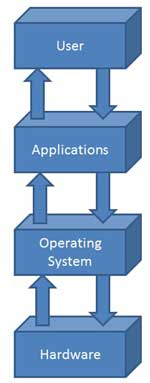
\includegraphics[scale=0.60]{images/os.png}\\
  \caption{Operating System}
  \label{fig1}
\end{figure}
\end{center}
\end{frame}

\begin{frame}
\frametitle{The principal tasks for an OS}
\begin{itemize}
    \item Processor (CPU) Management
    \item Memory (Storage) Management
    \item Devices Management
    \item Application Management
    \item User Interface (UI)
\end{itemize}
\end{frame}

\subsection{Why Linux?}

\begin{frame}
\frametitle{What is Linux?}
A free and open-source UNIX-like operating system developed under 
the GNU General Public License (GPL).
\begin{itemize}
    \item Free and open source.
    \item More and more popular
    \item Portable: Supports most of the available computers
\end{itemize}
\end{frame}

\begin{frame}
\frametitle{A Short History of UNIX}
\begin{itemize}
    \item Prototype: \emph{Multics} by AT\&T Bell Lab, GE and MIT
    \item 1969, UNIX by Ken Thompson and Dennis Ritchie
    \item 1973 UNIX rewritten with C (unprecedented, providing portability)
    \item Berkeley UNIX (BSD UNIX)
    \item 1983, System V
    \item Commercial Products: SunOS, Solaris, HP-UX, AIX, SCO-UNIX
\end{itemize}
\end{frame}

\begin{frame}
\frametitle{Advantages of UNIX}
\begin{itemize}
    \item Unix is very simple
    \begin{itemize}
        \item UNIX systems implement only hundreds of system calls and
        \item have a straightforward, even basic design.
    \end{itemize}
    \item In UNIX, everything is a file, which unifies the manipulation
        of data and devices into a set of core system calls.
    \item Kernels and all related system utilities are written in C
    \item Fast process creation and unique \emph{fork()} system call.
    \item Providing simple yet robust IPC  primitives.
    \item Exhibiting clean layering, with a strong separation between policy (what to do) 
		and mechanism (how to do).
\end{itemize}
\end{frame}

\begin{frame}
\frametitle{A Short History of Linux (1)}
\begin{figure}
  \includegraphics[width=1.5in]{images/stallman.jpg}
 \includegraphics[width=1in]{images/gnu.png}\\
\end{figure}

\begin{itemize}
    \item 1984, \emph{Richard Stallman, GNU Project}
    \begin{itemize}
        \item \textcolor{red}{GNU's Not Unix}:\url{http://www.gnu.org}
        \item \textcolor{red}{Copyleft}
    \end{itemize}
    \item Purpose: \emph{Free UNIX}
    \begin{itemize}
        \item \emph{Free as free speech, not free lunch.}
    \end{itemize}
    \item 1st step: re-implementation of UNIX utilities, especially
    \begin{itemize}
        \item C Compiler, C library
        \item emacs/bash
    \end{itemize}
    \item To fund the GNU project - Free Software Foundation (FSF)
    \begin{itemize}
        \item \url{http://www.fsf.org}
    \end{itemize}
\end{itemize}
\end{frame}

\begin{frame}
\frametitle{A Short History of Linux (2)}
\begin{figure}
  \includegraphics[width=.80in]{images/linus.jpg}
  \includegraphics[width=1in]{images/redhat.jpg}
\end{figure}

\begin{itemize}
    \item 1991, \emph{Linus Torvalds}, 1st version of \emph{Linux Kernel}
    \begin{itemize}
        \item Initially on the 386 protected mode
        \item Linus's UNIX = Linux
    \end{itemize}
    \item 1992: 1st distributions emerged
    \begin{itemize}
        \item Linux Kernel
        \item GNU and other tools
        \item Installation procedure
    \end{itemize}
    \item The rest is well-known history ...
    \begin{itemize}
        \item RedHat, Ubuntu, Debian, OpenSuSe, etc.
    \end{itemize}
\end{itemize}
\end{frame}

\begin{frame}
\frametitle{A Typical Computer System Architecture}
\begin{figure}
  \includegraphics[width=3in]{images/system.png}
\end{figure}
\end{frame}

\begin{frame}
\frametitle{Programmer's Viewpoint}
\begin{figure}
  \includegraphics[width=3in]{images/programmer.png}
\end{figure}
\end{frame}

\subsection{Future Perspectives}
\begin{frame}
\frametitle{Future Perspectives}
\begin{figure}
  \includegraphics[width=3in]{images/bulls.png}
\end{figure}
\end{frame}

\subsection{Basic Knowledge}

\begin{frame}
\frametitle{2-M: Multi-User and Multi-tasking}
\begin{itemize}
    \item Linux is a multi-user, multi-tasking OS
    \begin{itemize}
        \item Multiple users can run multiple tasks simultaneously, independent 
			of each other.
    \end{itemize}
    \item Always need to ``log in'' before using the system
    \begin{itemize}
        \item Identify yourself with username + password
    \end{itemize}
    \item Ways to log in to the system
    \begin{itemize}
        \item Console: Directly attached keyboard, mouse, monitor
        \item Serial terminal
        \item Network connection (ssh, telnet, etc.)
    \end{itemize}
\end{itemize}
\end{frame}

\subsection{Linux Commands}
\begin{frame}
\frametitle{Linux Commands}
\begin{itemize}
    \item Many things on a Linux system can be done by typing commands
    \item \textcolor{red}{Note that the GUI (X-window) is not needed for running a Linux system.}
    \item In order to type commands in X-window you need to start a terminal emulator
    \item Command Prompt
    \begin{itemize}
        \item Can be configure yourself, the default is
        \item \$ - ``logged in as a regular user''
        \item \# - ``logged in as root (privileged user)''
    \end{itemize}
\end{itemize}
\end{frame}

\begin{frame}
\frametitle{Start Linux}
\Large Now start Linux and log in as administrator ``root''; and then open a 
	terminal on your desktop. See, what's your command prompt?
\end{frame}

\begin{frame}[t,fragile]
\frametitle{Command Syntax}
\begin{block}{Syntax format}
\begin{quote}
<command> [option(s)] [argument(s)]
\end{quote}
\end{block}

\begin{block}{Examples}
\begin{lstlisting}
# list files and directories in current directory
ls
# list files and directories lengthily
ls -l
# list files and directories in /dev
ls /dev
ls -al /dev
\end{lstlisting}
\end{block}
\end{frame}

\begin{frame}
\frametitle{Some Useful Commands}
\begin{itemize}
    \item \textbf{passwd}: Change your password
    \item \textbf{mkpasswd}: Generate a random password
    \item \textbf{date, cal}: Find out today's date and display a calendar
    \item \textbf{who, finger}: Find out who else is active on the system
    \item \textbf{clear}: Clear the screen
    \item \textbf{echo}: Write a message to your screen
    \item \textbf{write, wall, talk, mesg}: Inter-user communication
    \item ...
\end{itemize}
\end{frame}

\begin{frame}
\frametitle{who, what, where, where to go}
\begin{itemize}
    \item \textbf{pwd}: Print Working Directory
    \item \textbf{uname}: Print the system information
    \item \textbf{whoami}: Who am I
    \item \textbf{cd}: Change Directory
\end{itemize}
\end{frame}

\begin{frame}
\frametitle{pwd: knowing where you are now}
\begin{itemize}
    \item \textbf{Synopsis}: \texttt{pwd}
    \item All the path names are started with a slash (``/''), for example
    \item ``/root'' is the home directory for root
    \item ``/home/xxx'' is the home directory for user ``xxx''
    \item Use command ``which pwd'' can show you where your command locates
    \item Most of the user commands are stored in \textcolor{red}{/bin} or \textcolor{red}{/usr/bin}
    \item Commands for super user are in the directories \textcolor{red}{/sbin} and \textcolor{red}{/usr/sbin}
\end{itemize}
\end{frame}

\begin{frame}
\frametitle{uname: knowing what my system is}
\begin{itemize}
    \item \textbf{Synopsis}: \texttt{uname option(s)}
    \item \texttt{uname -a: --all}
    \item \texttt{uname -i: --hardware-platform}
    \item \texttt{uname -m: --machine}
    \item \texttt{uname -n: --node-name}
    \item \texttt{uname -o: --operation-system}
    \item \texttt{uname -r: --kernel-release}
    \item \texttt{uname -s: --kernel-name}
    \item \texttt{uname -v: --kernel-version}
    \item \texttt{uname -p: --processor}
    \item You can use \texttt{uname --help} to obtain more information for this command.
    \item \color{blue!80}{This command is very useful in
compiling the system-dependent code.}
\end{itemize}
\end{frame}

\begin{frame}
\frametitle{whoami: knowing who you are}
\begin{itemize}
    \item \textbf{Synopsis}: \texttt{whoami}
    \item The command is different from ``who am i''
    \item and also ``who''
    \item Now guess what the command ``who'' can do for you?
\end{itemize}
\end{frame}

\begin{frame}
\frametitle{cd: change directory to}
\begin{itemize}
    \item \textbf{Synopsis}: \texttt{cd dir\_name}
    \item Command ``cd'' without any argument will direct you to your home directory
    \item Command ``cd $\sim$xxx'' can direct you to the home directory of user ``xxx''
    \item You can use either \textcolor{red}{absolute pathname} to visit the directory, e.g. ``cd /tmp'' or
    \item You can also use \textcolor{red}{relative pathname} to visit the relevant directory.
    \item If you are root, you can visit anywhere; but if you are a normal user, maybe you will be
        forbidden to visit somewhere, for example ``/root''.
\end{itemize}
\end{frame}

\begin{frame}
\frametitle{How to get help for a command}
\begin{itemize}
    \item ``man'' command
    \begin{itemize}
        \item for example ``man ls'' can return the manual for the command ``ls''
        \item manpage is stored in the directory/usr/share/man/
    \end{itemize}
    \item \textcolor{gray}{``info''}
    \item \texttt{command --help} or \texttt{command -h}
    \item \textcolor{red}{HOWTO} Documentation
    \item Refer to \textcolor{red}{Internet}
\end{itemize}
\end{frame}

\begin{frame}
\frametitle{The man command (1)}
\begin{itemize}
    \item With the man command you can get the manual page of commands
    \item Manual pages are stored in /usr/man or /usr/share/man
    \item The manual page consists of:
    \begin{itemize}
        \item \textbf{NAME}: The name of the command and a online description
        \item \textbf{SYNOPSIS}: The syntax of the command
        \item \textbf{DESCRIPTION}: Explanation of how the command works and what it does
        \item \textbf{Files}: The files used by the command
        \item \textbf{Bugs}: Known bugs and errors
        \item \textbf{See also}: Other relevant commands
    \end{itemize}
\end{itemize}
\end{frame}

\begin{frame}
\frametitle{The man command (2)}
\begin{itemize}
    \item The ``-k'' option
    \begin{itemize}
        \item man -k print
    \end{itemize}
    \item Manual pages are divided into 8 sections:
    \begin{enumerate}
        \item User commands
        \item System calls
        \item Libc calls
        \item Devices
        \item File formats and protocols
        \item Games
        \item Conventions, macro packages and so forth
        \item System administration
    \end{enumerate}
    \item To select the correct section, add section number:
    \begin{itemize}
        \item man 1 passwd
        \item man 5 passwd
    \end{itemize}
\end{itemize}
\end{frame}

\begin{frame}
\frametitle{The info command}
\begin{itemize}
    \item \textbf{FUNCTION}: Read documentation, sometimes an alternative for manual pages
    \item Information for info is stored in /usr/info or /usr/share/info
    \item Some info commands:
    \begin{itemize}
        \item SPACE: next screen of text
        \item DELETE: previous screen of text
        \item n: next node
        \item p: previous node
        \item u: up node
        \item q: quit info
        \item TAB: skip to next menu item
    \end{itemize}
\end{itemize}
\end{frame}

\begin{frame}
\frametitle{Working with Files and Directories}
\begin{block}{What is a file?}
\begin{itemize}
    \item A collection of data
    \item An object that can be read from, or written to, or both.
    \item \emph{All the objects in Linux are files}
    \item A file has certain attributes include
    \begin{itemize}
        \item \textcolor{red}{File type}
        \item \textcolor{red}{Access permissions}
    \end{itemize}
\end{itemize}
\end{block}
\begin{block}{File Structure}
\begin{itemize}
    \item Generally: byte stream, record sequence, record tree
    \item In Linux: byte stream
\end{itemize}
\end{block}
\end{frame}

\begin{frame}
\frametitle{Directory Structure}
\begin{figure}
    \includegraphics[width=2.5in]{images/directory.png}
\end{figure}
\begin{itemize}
    \item Linux File System Standard: \url{http://www.pathname/fhs}
\end{itemize}
\end{frame}

\end{CJK*}
\end{document}
